\subsubsection{Polarized PDFs}
\label{sec:polPDFs}

The fitting framework outlined in Sec.~\ref{sec:unpPDFs} can be applied
to a determination of longitudinally polarised PDFs as well.
%
Here we delineate the aspects of the framework specific to the polarised
case, and give a review of current global polarised PDF fits.

\paragraph{General framework.}
%
Longitudinally-polarised PDFs are defined as the net amount of parton 
densities with spin aligned along ($\uparrow$) or opposite ($\downarrow$)
the polarisation direction of the parent nucleon
\begin{equation}
\Delta f(x,\mu^2) \equiv f^{\uparrow}(x,\mu^2) - f^{\downarrow}(x,\mu^2)
\,\mbox{,}
\ \ \ \ \ \ \ \ \ \
f=u,\bar{u},d,\bar{d},s,\bar{s},g
\,\mbox{.}
\label{eq:polPDFs}
\end{equation}
%
Their interest is mostly related to the
first moments of the singlet and gluon polarised PDFs
\begin{align}
\Delta\Sigma(\mu^2)
& =
\sum_{q}^{n_f}\int_0^1 dx 
\left[\Delta q(x, \mu^2) + \Delta\bar{q}(x, \mu^2)\right]
=
\sum_q^{n_f}\langle 1 \rangle_{q^+}
\\
\Delta G(\mu^2)
& =
\int_0^1 dx \Delta g(x,\mu^2)
=
\langle 1 \rangle_g
\,,
\label{eq:moments}
\end{align}
which can be interpreted~\cite{Leader:2013jra} as the nucleon spin fractions 
carried by quarks/antiquarks and gluons respectively.

As in the case of unpolarised PDFs, the dependence on the scale $\mu$ can 
be computed perturbatively by means of DGLAP evolution equations, 
Eq.~(\ref{eq:dglap}).
%
The unpolarised splitting kernels $P_{ij}$ should be replaced with their
polarised counterparts, $\Delta P_{ij}$, which have been recently computed 
up to NNLO~\cite{Moch:2014sna} in the $\overline{\rm MS}$ renormalisation 
scheme.
%
Small-$x$ evolution equations which resum powers of $\alpha_s\ln^2(1/x)$
in the polarisation-dependent evolution along with powers of $\alpha_s\ln(1/x)$
in the unpolarised evolution have been recently proposed using the formalism
of Wilson line-like operators~\cite{Kovchegov:2015pbl}.
%
Both numerical~\cite{Kovchegov:2016weo}
and analytical~\cite{Kovchegov:2016zex,Kovchegov:2017jxc}
solutions to these small-$x$ evolution equations have been derived
for the flavour singlet combination of polarised PDFs.

The dependence on the momentum fraction $x$, fixed by non-perturbative QCD 
dynamics, should satisfy some theoretical constraints.
%
First, PDFs must lead to positive cross sections: 
at leading order (LO), this implies that polarized 
PDFs are bounded by their unpolarized counterparts\footnote{Beyond LO, more 
complicate relations hold~\cite{Altarelli:1998gn}; however they have little
effect on PDFs.}, $|\Delta f(x,\mu^2)|\leq f(x,\mu^2)$.
%
Second, PDFs must be integrable: this corresponds to the assumption 
that the nucleon matrix element of the axial current for each flavor is finite.
%
Third, it follows from SU(2) and SU(3) flavor symmetry that 
the first moments of the nonsinglet $\mathcal{C}$-even PDF combinations,
$\Delta T_3=\Delta u^+ -\Delta d^+$ and 
$\Delta T_8 = \Delta u^+ +\Delta d^+ -2\Delta s^+$ 
(where $\Delta q^+=\Delta q+\Delta\bar{q}$, $q=u,d,s$), are respectively
related to the baryon octet $\beta$-decay constants, whose 
measured values values are~\cite{Olive:2016xmw}
\begin{align}
 a_3
 & =
 \int_0^1 dx \Delta T_3 
 = \langle 1\rangle_{u^+} - \langle 1\rangle_{d^+}  = 1.2701 \pm 0.0025\\
 a_8
 & =
 \int_0^1 dx \Delta T_8 
 = \langle 1 \rangle_{u^+} + \langle 1 \rangle_{d^+} -2\,\langle 1 \rangle_{s^+} 
 =0.585  \pm 0.025
 \,\mbox{.}
\label{eq:decayconst}
\end{align}
%
Fairly significant violations of SU(3) symmetry are advocated
in the literature (see {\it e.g.} Ref.~\cite{Cabibbo:2003cu} for a review). 
%
In this case, an uncertainty on the octet axial charge, 
larger up to $30\%$ than its experimental value in Eq.~\eqref{eq:decayconst}, 
is found~\cite{FloresMendieta:1998ii}. 

The bulk of the experimental information on polarized PDFs comes from 
neutral-current inclusive and semi-inclusive Deep-Inelastic Scattering 
(DIS and SIDIS) with charged lepton beams and nuclear targets. 
%
Because of the way the corresponding observables factorise, inclusive DIS 
data constrain the total quark combinations $\Delta q^+$ only, 
while SIDIS data with identified pions or kaons in the final state 
constrain individual quark and antiquark flavours. 
%
In principle, both DIS and SIDIS are also sensitive to the gluon 
distribution $\Delta g$, as it directly enters the factorised expressions of
the corresponding structure functions beyond LO, and indirectly via DGLAP 
evolution.
%
In practice the constraining power of DIS and SIDIS data on $\Delta g$ is 
rather weak, because of the limited $Q^2$ range covered by the data. 

Note that, in the case of SIDIS, a reliable knowledge of 
Fragmentation Functions is required in the factorised expressions of the 
corresponding observables. 
%
Since FFs are non-perturbative objects on the 
same footing as PDFs, they are likely an additional source of 
bias in the PDF determination.
%
For this reason, a significant experimental and theoreticla effort has been
put in improving the independent determination of 
FFs~\cite{deFlorian:2014xna,deFlorian:2017lwf,
Hirai:2016loo,Sato:2016tuz,Nocera:2017qgb,Bertone:2017xsf}.

Beside DIS and SIDIS fixed-target data, a significant amount of data from
longitudinally polarized proton-proton ($pp$) collisions at the Relativistic 
Heavy Ion Collider (RHIC) have become available recently (see {\it e.g.} 
Ref.~\cite{Aschenauer:2015eha}for an overview), although in a limited range 
of momentum fractions, $0.05\lesssim x \lesssim 0.4$.
%
On the one hand, longitudinal (parity-violating) single-spin and 
(parity-conserving) double-spin asymmetries for $W^\pm$ boson production are 
sensitive to the flavor decomposition of polarized quark and antiquark 
distributions, because of the chiral nature of the weak 
interactions~\cite{Bourrely:1993dd}. 
%
On the other hand, double-spin asymmetries for jet, di-jet and $\pi^0$ 
production are directly sensitive to the gluon polarization in 
the proton, because of the dominance of gluon-gluon and quark-gluon initiated 
subprocesses in the kinematic range accessed by RHIC~\cite{Bourrely:1990pz}.

The kinematic coverage of the data which can be used to constrain polarised 
PDFs is displayed in Fig.~\ref{fig:kinEIC}.
%
By comparison with Fig.~\ref{fig:kinplot-report}, it is apparent that the
quantity of data points, their kinematic coverage and the variety of 
available hard-scattering processes are much more limited in the polarised case
than in teh unpolarised case.
%
Therefore polarised PDFs can currently be determined with much less 
precision than their unpolarised counterparts.
%
The kinematic coverage is expected to be significantly extended in the future,
with DIS and SIDIS data from JLab-12~\cite{Dudek:2012vr} and a polarised 
high-energy Electron-Ion Collider (EIC)~\cite{Accardi:2012qut}.
%
Such an extended kinematic coverage is also displayed on Fig.\ref{fig:kinEIC}.
%
The eRHIC realisation of an EIC~\cite{Aschenauer:2014cki} has been considered.

%-------------------------------------------------------------------------------
\begin{figure}[!t]
\centering
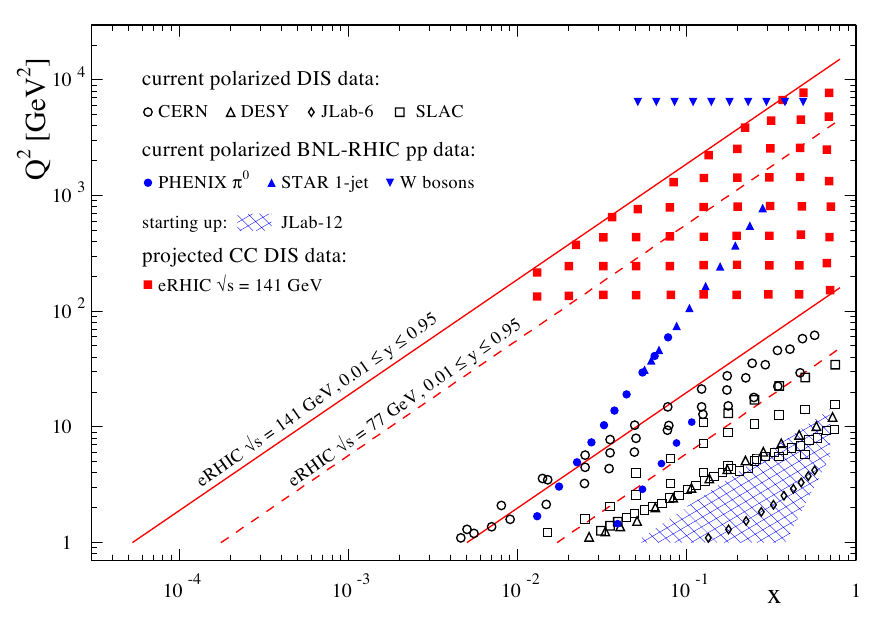
\includegraphics[width=0.9\textwidth]{plots/kinEIC}\\
\caption{\small Representative kinematic coverage, in the $(x,Q^2)$ plane,
of the (neutral current) DIS, SIDIS and $pp$ hard-scattering measurements 
that are used as input in a global polarised PDF fit.
%
The extended kinematic coverage achieved by 
JLab-12~\cite{Dudek:2012vr} and by the eRHIC~\cite{Aschenauer:2014cki} 
realisation of an EIC~\cite{Accardi:2012qut}
(including projected charged-current (CC) DIS data) is also shown.
%
Figure taken from Ref.~\cite{Aschenauer:2014cki}.}
\label{fig:kinEIC}
\end{figure}
%-------------------------------------------------------------------------------

A representative illustration of polarised PDFs obtained from a global
QCD analysis, namely NNDPFpol1.1, is provided in Fig.~\ref{fig:qPDFpol}.
%
The format is the same as for the unpolarised case, Fig.~\ref{fig:nnlopdfs},
in order to ease any comparison between the two.
%
In particular, note the suppression of all polarised PDFs at small values of 
$x$, including polarised sea quark PDFs, with respect to their unpolarised 
counterparts.
%
This is a consequence of the different structure of the polarised and 
unpolarised splitting functions in the DGLAP evolution equations. 

%-------------------------------------------------------------------------------
\begin{figure}[!t]
\centering
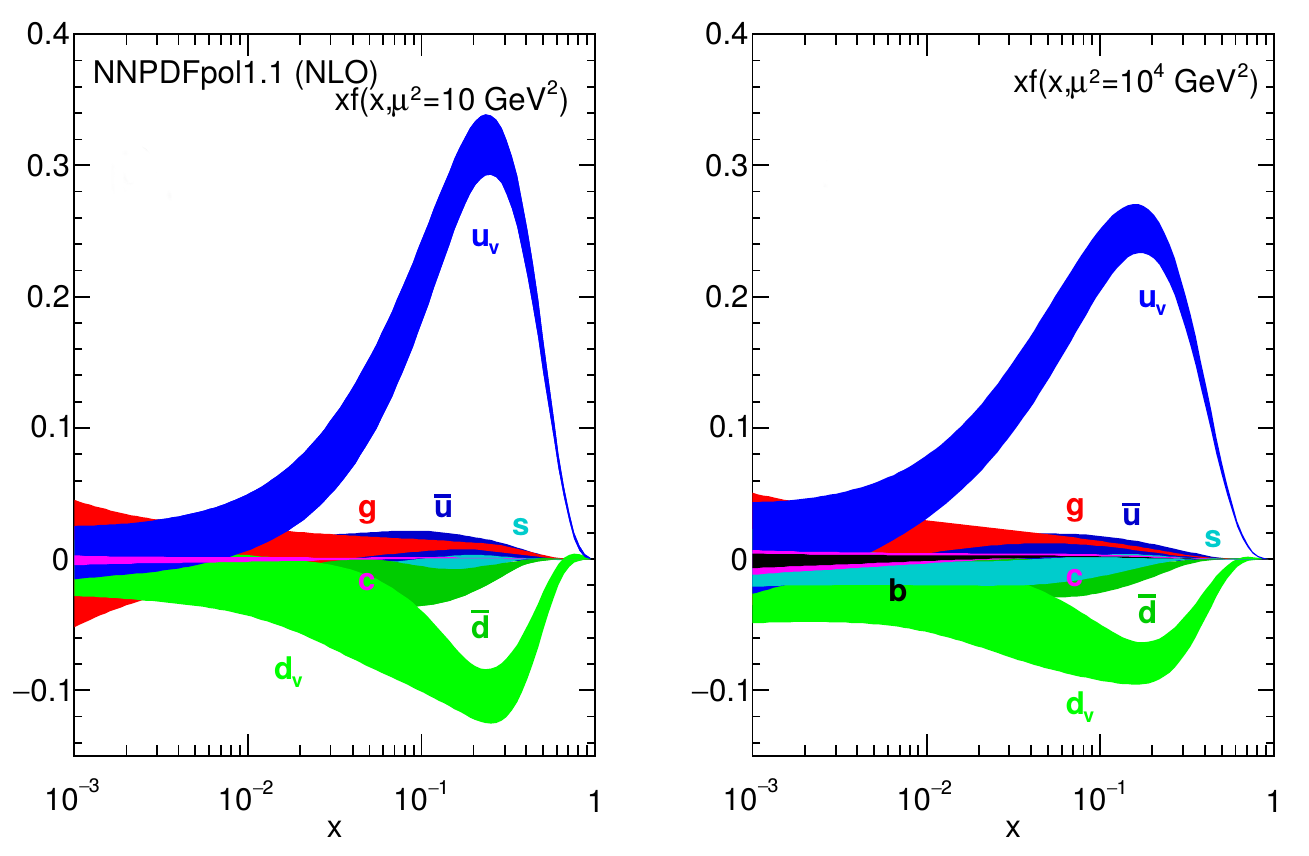
\includegraphics[scale=0.4]{plots/NNPDFpol}\\
\caption{\small Same as Fig.~\ref{fig:nnlopdfs}, 
but for the polarised NNPDFpol1.1 NLO PDFs.}
\label{fig:qPDFpol}
\end{figure}
%-------------------------------------------------------------------------------

\paragraph{State-of-the-art global polarised PDF fits.}

Several determinations of polarized PDFs of the proton (up to 
NLO\footnote{A NNLO QCD analysis of polarised PDFs based on inclusive DIS
data only was performed in Refs.~\cite{Shahri:2016uzl,Khanpour:2017cha}.
Inclusive DIS is the only polarised process for which coefficient functions
are known up to NNLO (all others are known only up to NLO).} 
and mostly 
in the $\overline{\rm MS}$ factorization scheme) are available in the 
literature, aiming at unveiling how much large and uncertain are 
$\Delta\Sigma$ and  $\Delta G$, Eq.~\eqref{eq:moments}. 
%
They differ among each other for the data set included in the analysis,
for some details of the QCD analysis (like the treatment of higher-twist
corrections) and for the procedure used to determine PDFs from the data 
(for details, see {\it e.g.} Chap.~3 in Ref.~\cite{Nocera:2014vla} 
and Ref.~\cite{Nocera:2016xhb}). 
%
In this respect, beside the standard and NNDPF
procedures outlined in Sec.~\ref{sec:unpPDFs},
an iterative Monte Carlo procedure has been developed by the JAM
collaboration~\cite{Sato:2016tuz}.

In particular, motivated by the interest in studying the effects RHIC $pp$ 
data, two new global analyses of polarized PDFs have been carried out in
2014, DSSV14~\cite{deFlorian:2014yva} and NNPDFpol1.1~\cite{Nocera:2014gqa},
based respectively on the standard and NNPDF methodologies outlined 
in Sec.~\ref{sec:unpPDFs}.
%
These upgrade the corresponding previous analyses, 
DSSV08~\cite{deFlorian:2008mr} and 
NNPDFpol1.0~\cite{Ball:2013lla}, with data respectively on double-spin 
asymmetries for inclusive jet production~\cite{Adamczyk:2014ozi} 
and $\pi^0$ production~\cite{Adare:2014hsq}\footnote{Preliminary RHIC results 
included in Ref.~\cite{deFlorian:2008mr} were replaced in
Ref.~\cite{deFlorian:2014yva} with final results.}, 
and on double-spin asymmetries for high-$p_T$ inclusive jet 
production~\cite{Adamczyk:2014ozi,Adamczyk:2012qj,Adare:2010cc} and single-spin
asymmetries for $W^\pm$ production~\cite{Adamczyk:2014xyw}.
%
The new data have been included in NNPDFpol1.1 
by means of Bayesian reweighting~\cite{Ball:2010gb},
and in DSSV14 by means of a full refit.  

Overall, both the DSSV14 and NNPDFpol1.1 PDF determinations are 
state-of-the-art in the inclusion of the available experimental information. 
%
The data sets in the two analyses differ between each other only for 
fixed-target SIDIS and RHIC $\pi^0$ production measurements, included in 
DSSV14, but not in NNPDFpol1.1. 
%
The information brought in by these data is complementary to that provided by 
RHIC $W^\pm$ production and inclusive jet production data respectively. 

The effect of RHIC data on the polarized PDFs of the proton is twofold. 
 
\begin{itemize}

\item The 2012 STAR data sets on $W$ production~\cite{Adamczyk:2014xyw}, 
included in NNPDFpol1.1, provide evidence of a positive 
$\Delta\bar{u}$ distribution 
and a negative $\Delta\bar{d}$ distribution, with 
$|\Delta\bar{d}|>|\Delta\bar{u}|$~\cite{Nocera:2014gqa}.
% 
The size of the flavor symmetry breaking for polarized sea quarks is 
quantified by the asymmetry $\Delta\bar{u}-\Delta\bar{d}$, which,
in the NNPDFpol1.1 analysis, turned out to be roughly as large as its 
unpolarized counterpart (in absolute value), 
though much more uncertain~\cite{Nocera:2014rea}. 
%
Even within this uncertainty,
polarized and unpolarized light sea quark asymmetries show opposite sings,
with the polarized being definitely positive.  
%
This result may discriminate between one model of nucleon structure and 
another, see left panel of Fig.~\ref{fig:RHICpdfs}: 
specifically, some meson-cloud (MC) models are disfavored, while a more 
accurate experimental information is needed to establish whether 
chiral quark-soliton (CQS), Pauli-blocking (PB) or statistical (ST)
models are preferred (these models are described in 
Ref.~\cite{Chang:2014jba}).

\item The 2009 STAR and PHENIX data sets on jet and $\pi^0$ 
production~\cite{Adamczyk:2014ozi,Adare:2014hsq}, included in DSSV14
and NNPDFpol1.1, provide first the evidence
of a sizable positive gluon polarization in the proton. 
%
A comparison of the gluon PDF in the two PDF sets is displayed in 
Fig.~\ref{fig:RHICpdfs} (right panel). 
%
Comparable results, both central values and uncertainties, are found in the 
$x$ region covered by RHIC data. 
%
The agreement between the two analyses is optimal in the
range $0.08\leq x \leq 0.2$, where the dominant experimental information comes
from jet data; a slightly smaller central value is found in the DSSV14 
analysis, in comparison to the NNPDFpol1.1, in the range 
$0.05\leq x \leq 0.08$, where the dominant experimental information comes from 
$\pi^0$ production data. 
%
Indeed, these are included in DSSV14 but are not
in NNPDFpol1.1. 
%
Nevertheless, best fits lie well within each other error
bands, though NNPDFpol1.1 uncertainties tend to be larger than DSSV14
uncertainties outside the region covered by RHIC data.
%
Very well compatible values of the integral of $\Delta g$, 
Eq.~\eqref{eq:moments}, truncated over the interval $0.05\leq x \leq 1$, are 
found: at $Q^2=10$ GeV$^2$, this is $0.20^{+0.06}_{-0.07}$ for 
DSSV14~\cite{deFlorian:2014yva}, and $0.23\pm 0.06$ for 
NNPDFpol1.1~\cite{Nocera:2014gqa}.
\end{itemize}

%------------------------------------------------------------------------------
\begin{figure}[!t]
\centering
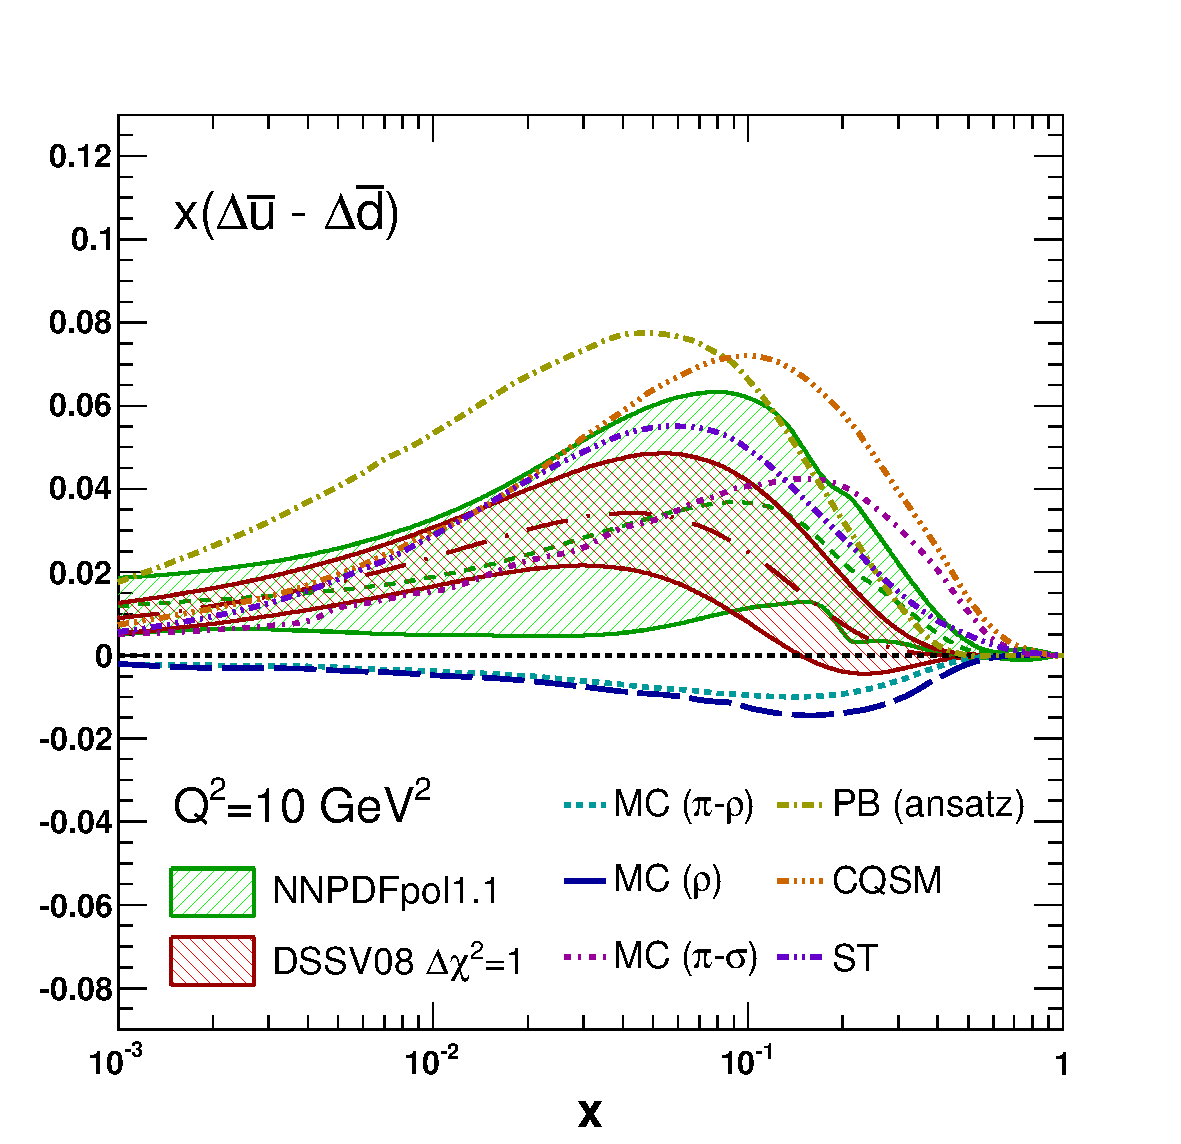
\includegraphics[scale=0.35]{plots/asysea_2}
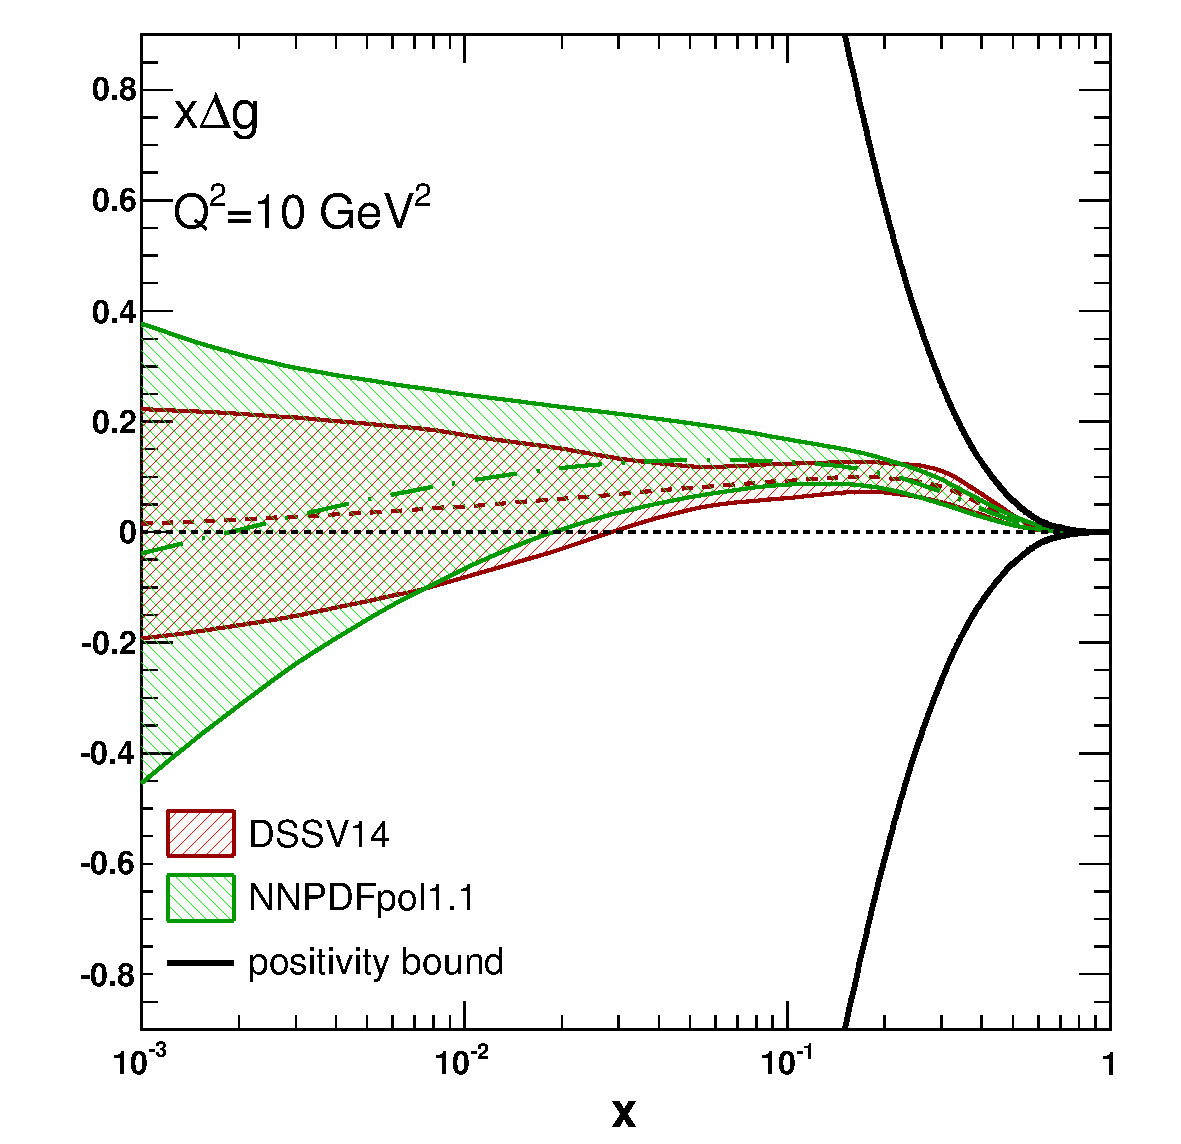
\includegraphics[scale=0.325]{plots/gluoncomp}\\
\caption{(Left) The polarized light sea quark asymmetry 
$x(\Delta\bar{u}-\Delta\bar{d})$ from the NNPDFpol1.1 and 
DSSV08 PDF sets at $Q^2=10$ GeV$^2$, compared to expectations from 
various models of nucleon structure~\cite{Chang:2014jba}. 
(Right) The polarized gluon $x\Delta g$ from the 
DSSV14 and NNPDFpol1.1 PDF sets at $Q^2=10$ GeV$^2$.}
\label{fig:RHICpdfs}
\end{figure}
%------------------------------------------------------------------------------

\paragraph{Open issues.}

Despite the achievements described above, polarised PDFs cannot be determined 
in a global QCD analysis with the same accuracy as their unpolarised 
counterparts.

\begin{itemize}

\item Experimental data are lacking over a wide range of $x$ and $Q^2$.
%
As a consequence, the size of the contribution of quarks, antiquarks and 
gluons to the nucleon spin, as quantified by their first moments, 
Eq.~\eqref{eq:moments}, is affected by large uncertainties. 
%
These come predominantly from the extrapolation into the small-$x$ region 
($x\lesssim 10^{-3}$), not covered by experimental data, where, for
instance, modified small-$x$ evolution cannot be tested.
%
The limited range in $Q^2$ is also a limiting factor in the determiantion
of $\Delta g$ via evolution.
%
Likewise, extrapolation uncertainties in the large-$x$ region
($x\gtrsim 0.7$) do not allow one to investigate for instance
the behaviour of ratios of light polarised to unpolarised PDFs.
%
Such a behaviour is predicted in several nonperturbative models
of nucleon structure, and is often related to first QCD principles,
like fundamental symmetries (for a comparison between PDF and 
model preditions, see Ref.~\cite{Nocera:2014uea}).

\item Inclusive DIS data, together with nonsinglet axial couplings, 
Eq.~\eqref{eq:decayconst}, and kaon SIDIS data provide the sole available 
constraint on the total strange distribution $\Delta s^+$.
%
A sizeable negative polarised $\Delta s^+$ distribution is found 
consistently in all analyses based on inclusive DIS data only.
%
However, the shape of $\Delta s^+$ may vary significantly in anlyses based
also on SIDIS data, typically depending on the set of kaon FFs used to compute
the corresponding observables~\cite{Leader:2011tm}.
%
This issue has been recently clarified in Ref.~\cite{Ethier:2017zbq},
where a simultaneous determination of polarised PDFs and unpolarised PDFs
hahs been performed based on DIS, SIDIS and single-inclusive annihilation data.
%
Moreover, in order to avoid biasing the determination of $\Delta s^+$ by 
assumptions on SU(3) symmetry, the data alone are allowed to determine the 
octet axial charge in Eq.~(\ref{eq:decayconst}).
%
This translates into a slightly positive $\Delta s^+$ distribution,
although with inflated uncertainties compatible with the negative result 
found from inclusive DIS, and into an octet axial charge about $20\%$ 
smaller than its quoted experimental value, Eq.~(\ref{eq:decayconst}).
%
Further higher precision kaon SIDIS data would be needed in order to reduce 
the uncertainty on $\Delta s^+$ and test the degree of SU(3) breaking.

\end{itemize}

Ongoing and future experimental campaigns at current facilities are
expected to provide an additional piece of experimental information
in order to address some of the issues outlined above (for an 
assessment of the impact of very recent/forthcoming data, see {\it e.g.}
Refs.~\cite{Aschenauer:2015eha,Aschenauer:2015ata,Nocera:2015vva,
Nocera:2017wep}).
%
However, a future high-energy, polarized EIC~\cite{Accardi:2012qut} will 
likely be the only facility to address all the above questions with the 
highest precision. 
% 
The extension of the kinematic reach down to $x\sim 10^{-4}$ and up to
$Q^2=10^4$ GeV$^2$ will allow for an accurate determination of $\Delta g$
via scaling violations in inclusive DIS, of $\Delta\bar{u}$ and 
$\Delta\bar{d}$ via inclusive DIS at high $Q^2$ mediated by electroweak bosons,
and of $\Delta s$ via kaon-tagged SIDIS. 
%
The expected impact of a longitudianlly polarised program at an EIC
have been quantitatively assessed in several dedicated 
studies~\cite{Aschenauer:2012ve,Ball:2013tyh,Aschenauer:2013iia,
Aschenauer:2015ata}.
